\chapter{The human microbiome and non-alcoholic fatty liver disease}

\section{Introduction}
Non alcoholic fatty liver disease (NAFLD) has been on the rise along with obesity, affecting a fifth to a third of the North American population \cite{preiss2008non}. Most people with NAFLD remain asymptomatic, however, in up to a third of patients NAFLD can progress to non-alcoholic steatohepatitis (NASH), causing inflammation and scarring in the liver, and decreasing the 5 year survival rate to 67\% \cite{propst1995prognosis}. If we can shed some light on the process by which people progress from NAFLD to NASH, we might be able to find treatments to prevent NASH.

There are several known genetic factors that increase the risk of progression to NASH. The I148M variant of the Patatin-Like Phospholipase Domain Containing 3 gene (PNPLA3) correlates with a 3.2 fold increased risk of NASH from NAFLD when present homozygously, compared to to patients without the variant \cite{sookoian2011meta}. Additionally, mice with a toll-like receptor 4 knockout had lower lipid and injury accumulation markers when fed a methionine/choline-deficient diet which would normally induce steatohepatitis in wild type mice \cite{rivera2007toll}.

On the epigenetic level, genes are differentially methylated in advanced NAFLD compared to mild NAFLD. 11\% of genes are differentially hypomethylated in advanced NAFLD (compared to 3\% hypermethylated), leading to increased expression \cite{murphy2013relationship}. On a hormonal level, estrogen has been shown to inhibit fibrosis in rats \cite{yasuda1999suppressive}. On a metabolite level, Raman et al. found differences in the number of volatile organic compounds detected in patients with NAFLD compared to obese patients without NAFLD \cite{raman2013fecal}. Reactive oxygen species have also been implicated in NASH due to their involvement in the mechanism of steatohepatitis-inducing drugs \cite{berson1998steatohepatitis}.

A 2001 paper performed C-D-xylose-lactulose breath tests and measured tumor necrosis factor alpha levels to determine presence of bacterial overgrowth, and found increased bacterial overgrowth in 22 patients with NASH compared to 23 healthy controls \cite{wigg2001role}. Some papers claim a link between ethanol-producing gut bacteria and NAFLD \cite{zhu2013characterization} \cite{jiang2015dysbiosis}, however, no multiple test correction was performed in these studies.

Several papers have already been published in the literature on the topic of NAFLD and the gut microbiome:

\begin{figure}[h]
\begin{center}
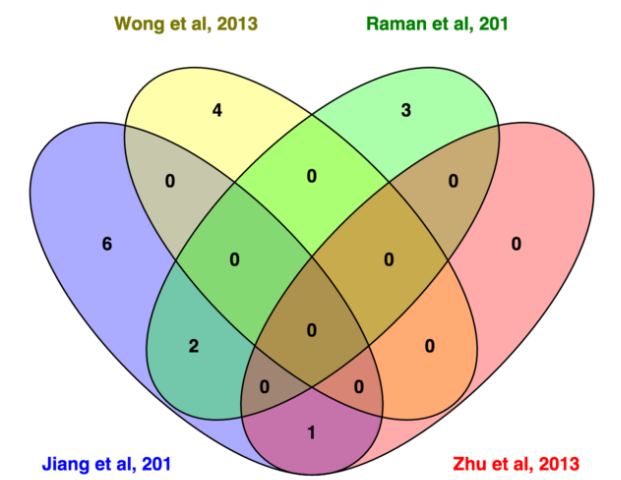
\includegraphics[width=0.7\textwidth]{nafld_papers.png}
\caption{\textbf{Venn diagram of genus found to be differentially abundant by different studies between NASH/NAFLD and healthy controls.} Boursier et al 2015 is not included as they reported a p-value of less than 0.05 for the Bacteroides genus only, which was not reported in any of the other studies. Only 3 out of the 16 genus claimed to be differentially abundant were the same in two studies: Escherichia was found in the Zhu \cite{zhu2013characterization} and Jiang \cite{jiang2015dysbiosis} studies, and Lactobacillus and Oscillibacter were found in the Jiang \cite{jiang2015dysbiosis} and Raman \cite{raman2013fecal} studies.}
\end{center}
\end{figure}

\begin{itemize}
\item Jiang et al, 2015 \cite{jiang2015dysbiosis} compared 53 NAFLD patients with 32 healthy controls

\item Zhu et al, 2013 \cite{zhu2013characterization} compared 16 non-obese controls, 25 obese patients, and 22 NASH patients

\item Raman et al, 2013 \cite{raman2013fecal} compared 30 NAFLD patients with 30 healthy controls

\item Wong et al, 2013 \cite{wong2013molecular} compared 16 NASH patients with 22 healthy controls

\item Boursier et al, 2015 \cite{boursier2016severity} compared 30 patients with F0 or F1 fibrosis to 27 patients with F2 or greater fibrosis, 35 of which had NASH
\end{itemize}

Of these, only Raman et al \cite{raman2013fecal} reported using a multiple test correction.

These five studies do not form a consistent story about the gut microbiome and NAFLD. We hope to run our own analysis rigorously, such that our results are replicable. Additionally, we are running a deeply sequenced metagenomic study, which hasn’t been done in the past.

\FloatBarrier

\section{Methods}
In total, 92 samples were collected: 41 from patients with NASH, 18 from patients with SS, and 33 from healthy controls.

[TO DO: include information about sample collection and exclusion criteria]

DNA extraction was performed with the \href{http://omegabiotek.com/store/product/stool-dna-kit/}{E.Z.N.A.® Stool DNA Kit}, and the protocol was followed with the addition of lysozyme with an extra 30 minute incubation at 37 degrees Celcius, between steps 2 and 3.

\subsection{16S rRNA gene tag experiment}

DNA was amplified by PCR according to the Earth Microbiome protocol \cite{caporaso2012ultra}, with the addition of barcodes so that all the samples could be sequenced in the same sequencing run \cite{gloor2010microbiome}. The DNA was sequenced on the Illumina MiSeq platform with paired end 150 nucleotide reads, producing 34955148 reads in total.

Reads were overlapped with Pandaseq \cite{masella2012pandaseq}, clustered into Operational Taxonomic Units using UCLUST \cite{edgar2010search}, and annotated with the SILVA database \cite{quast2013silva}, producing a table of counts per operational taxonomic unit per sample. 16809756 reads (48\%) were succesfully overlapped and annotated with 232 OTUs. Differential abudance was analyzed using ALDEx2 \cite{fernandes2014unifying}.

\subsection{Metagenomic experiment}

A deep metagenomic sequencing experiment was performed using samples from 10 healthy controls and 10 of the patients with NASH. Samples from healthy patients were selected to exclude confounding factors, such as having a different country of birth, which could affect diet. Samples from NASH patients were selected for the strongest NASH phenotype.

The DNA was sequenced on the Illumini HiSeq platform, with single end 100 nucleotide reads. Samples were barcoded and sequenced on the same sequencing run. After sequencing, the reads were quality filtered and demultiplexed to separate the reads for each sample, yielding 1914714572 reads in total.

To annotate the reads, we used a two pronged strategy:

First, we created a reference library using the inferred taxa from the 16S rRNA gene tag experiment. For each genus the OTUs were annotated with, we randomly picked 10 strain genomes from the NCBI bacterial genome database. For genus where there were less than 10 fully sequenced representatives, we selected all genomes available. The library was made with 1134 genomes from 104 bacterial genus. The library was then clustered at 99\% identity for each genus using CD-HIT \cite{li2006cd} to decrease the number of sequences in the library from 3495887 to 2256844. Annotation was performed with the SEED database \cite{overbeek2005subsystems}, and sequenced reads were mapped onto this library. Out of 1914714572 reads total, 585382507 (30.6\%) were annotated by this method, over 5836 unique SEED hierarchy annotations. The code for the \href{https://github.com/ruthgrace/make_functional_mapping_library}{reference library creation} and \href{https://github.com/ruthgrace/mapping_library_annotated_counts}{annotation} is on GitHub.

Second, we assembled the reads per sample de novo using Trinity \cite{haas2013novo}, producing 8847816 sequences, and removed sequences that matched our reference library with 90\% identity as determined by BLAST \cite{altschul1990basic}, leaving 5876423 sequences. [FILL IN THIS] of these assembled sequences were successfully annotated with the SEED database \cite{overbeek2005subsystems}, and sequenced reads were mapped onto this. [FILL IN THIS] additional reads were annotated by this method, over [FILL IN THIS] unique SEED hierarchy annotations. The code for the custom assembly pipeline is on \href{https://github.com/ruthgrace/exploring_nafld_assembly}{GitHub}. The data from both prongs was amalgamated into a single table of counts per annotation per sample.

Differential abudance was analyzed using ALDEx2 \cite{fernandes2014unifying}.

\section{Results}

\subsection{16S rRNA gene tag experiment}

[consider adding nice bar graphs]

\begin{figure}[h]
\begin{center}
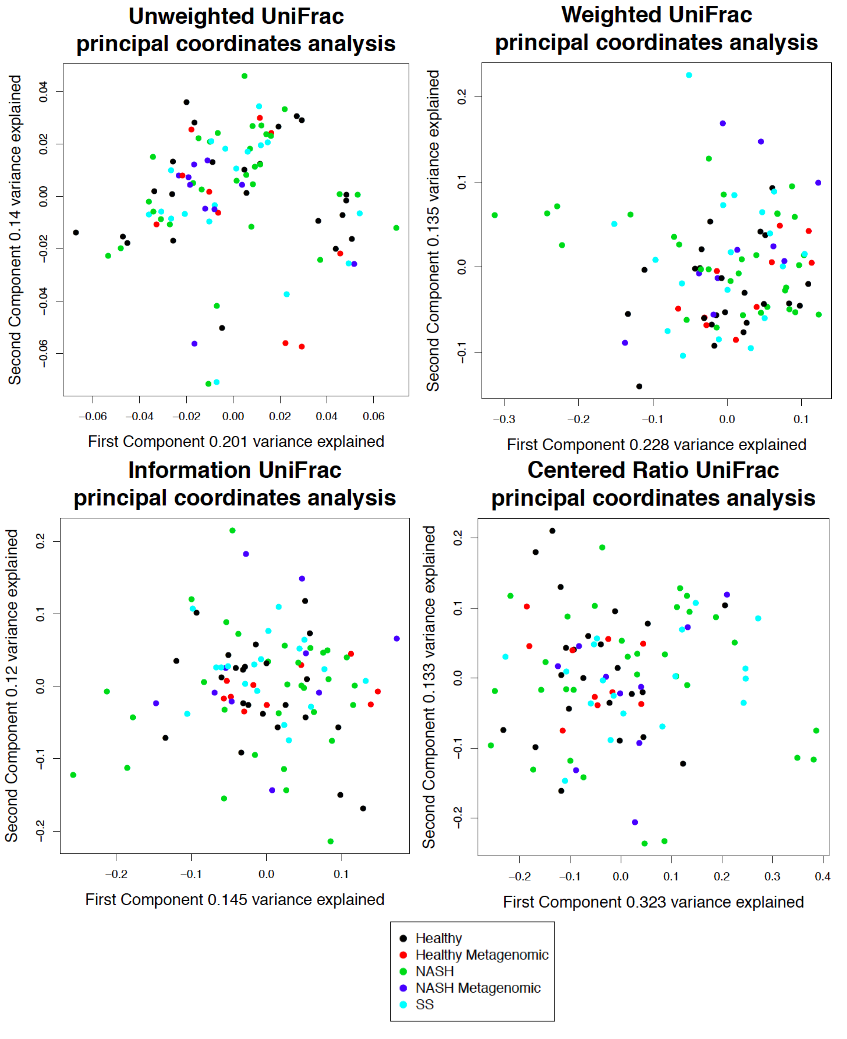
\includegraphics[width=0.7\textwidth]{nafld_16s_pcoa.png}
\caption{\textbf{Principal Components Analysis of 16S rRNA gene tag sequencing data with different UniFrac weightings.} Each point represents one sample, and the distances between the samples have been calculated using different UniFrac metrics, taking into account phylogenetic as well as abundance information. There is no obvious separation between groups by any of the UniFrac weightings. Furthermore the variance explained by each principal component axis is not notably high, indicating a rather uniform data set.}
\end{center}
\end{figure}



\begin{figure}[h]
\begin{center}
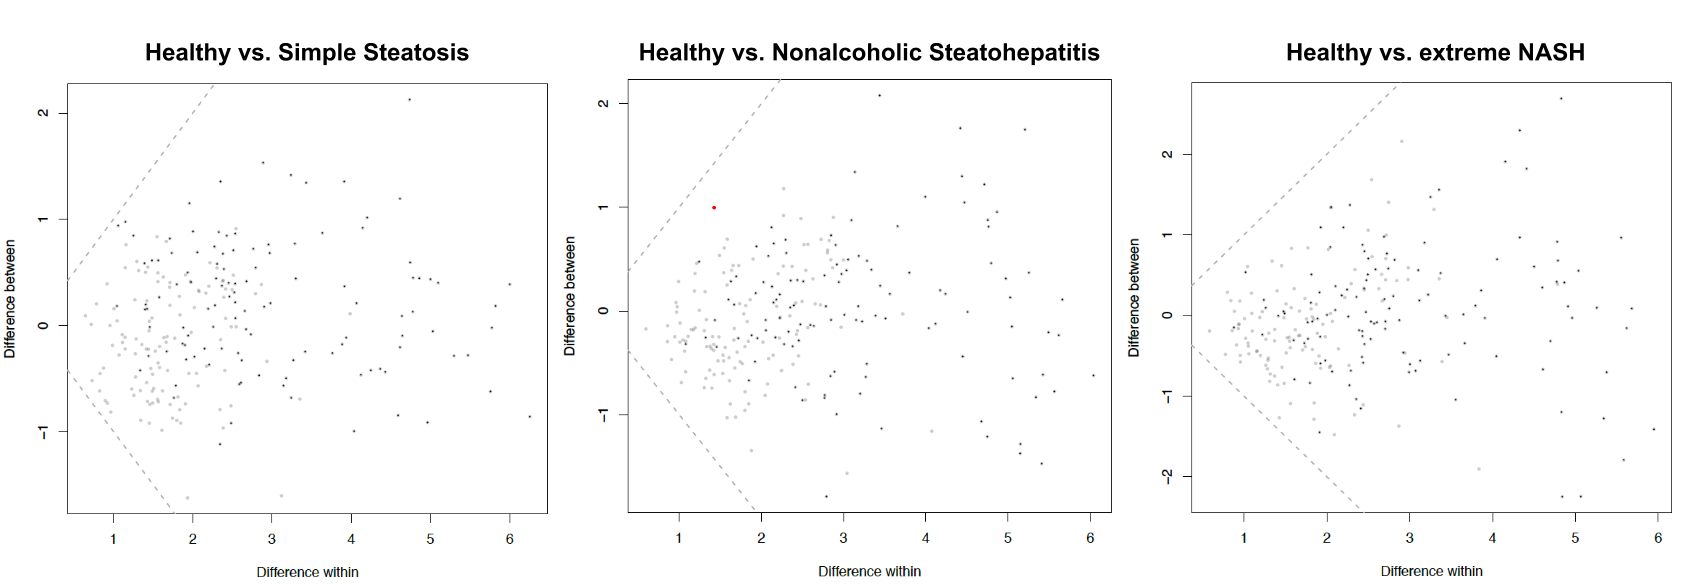
\includegraphics[width=0.7\textwidth]{nafld_16s_aldex.png}
\caption{\textbf{Difference within vs. difference between groups.} Each point represents one OTU, and the differential abundance of that OTU within groups is plotted against the differential abundance between groups. None of the OTUs are more different between groups than within groups. The healthy samples used for these comparisons are the 10 healthy samples used for the metagenomic study. The extreme NASH samples used for these comparisons are the subset of the NASH patients selected for the metegenomic study.}
\end{center}
\end{figure}

\begin{figure}[h]
\begin{center}
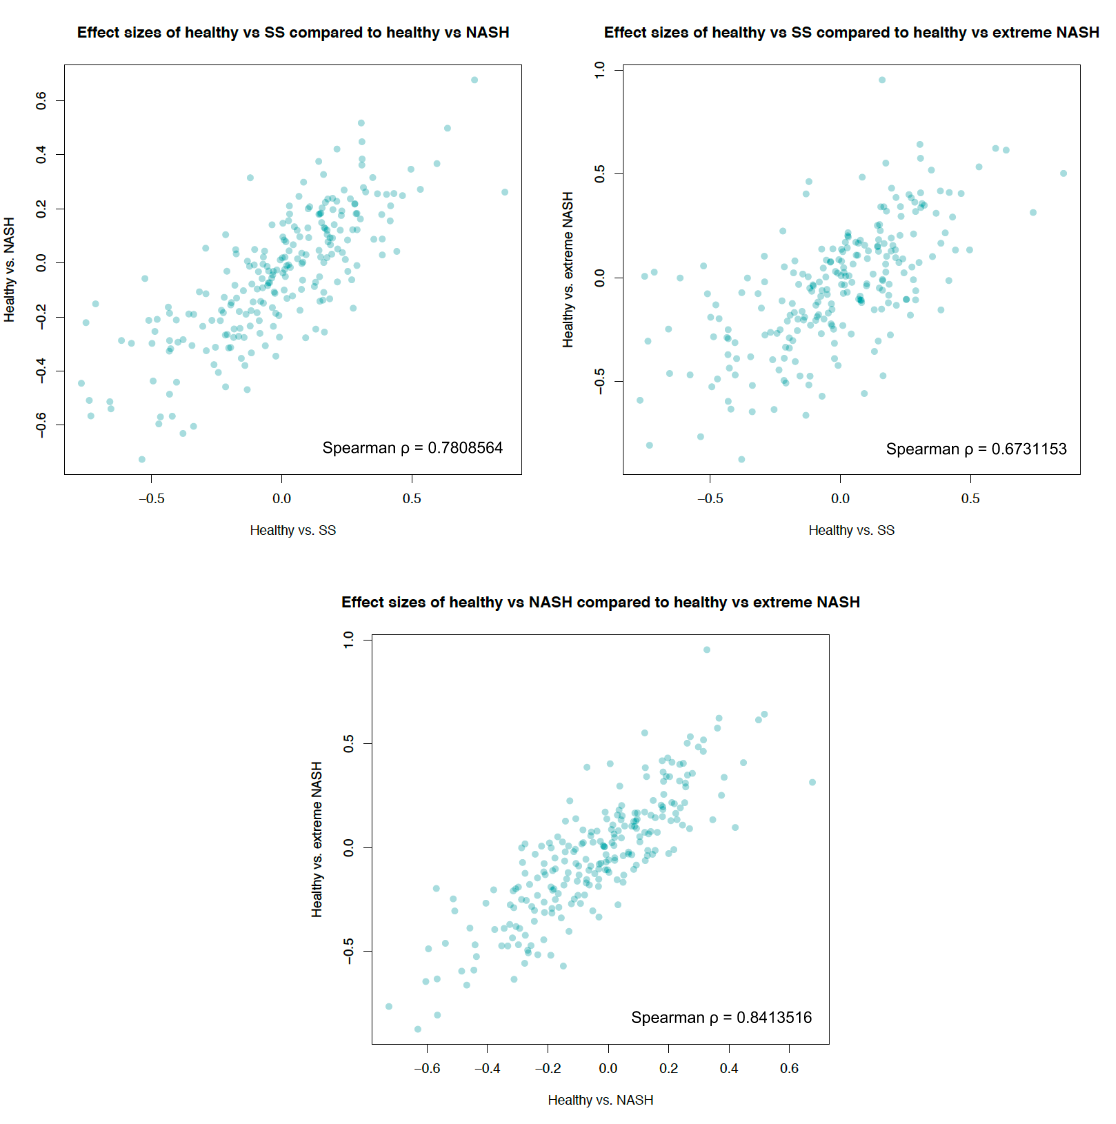
\includegraphics[width=0.7\textwidth]{nafld_16s_effect_sizes.png}
\caption{\textbf{Correlation in effect sizes of different group experiments.} Each point represents one OTU, and the effect size of that OTU in one comparison (for example, comparing the gut microbiome of healthy patients with patients who have simple steatosis) is plotted against the effect size of that OTU in another comparison. The healthy samples used for these comparisons are the 10 healthy samples used for the metagenomic study. The extreme NASH samples used for these comparisons are the subset of the NASH patients selected for the metegenomic study.}
\end{center}
\end{figure}

\subsection{Metagenomic experiment}

\section{Discussion}

From [cite figure], it appears that the effect sizes for 